% Final project report for the Marie Curie team
% Written by William Harrington
% ECE478 Final Project
\documentclass[12pt]{article}
\usepackage{amsmath}
\usepackage{amssymb}
\usepackage{graphicx}
\usepackage{tabulary}
\usepackage{float}
\usepackage{hyperref}
\usepackage{tikz}
\usetikzlibrary{arrows, decorations.markings}

\tikzstyle{vecArrow} = [thick, decoration={markings,mark=at position
   1 with {\arrow[semithick]{open triangle 60}}},
   double distance=1.4pt, shorten >= 5.5pt,
   preaction = {decorate},
   postaction = {draw,line width=1.4pt, white,shorten >= 4.5pt}]
\tikzstyle{innerWhite} = [semithick, white,line width=1.4pt, shorten >= 4.5pt]

\begin{document}

\title{Final Project}%replace X with the appropriate number
\author{William Harrington, Sheetal Konnur\\ %replace with your name
ECE478} %if necessary, replace with your course title
\date{}
 
\maketitle
\small
\begin{description}
	\item[Introduction] \hfill \\
		This report contains a detailed explanation of the Final project for the Marie Curie group. \\ \\
		\textbf{Goals}
		\begin{enumerate}
			\item Use an arduino to drive the servo controller
			\item Use a raspberry pi 2 to do image processing with a kinect
			\item Interface raspberry pi 2 and arduino
			\item Implement some sort of behavior in the robot based on
			\item Add mechanical support for shoulders
		\end{enumerate}
		\centering
		\tikzstyle{int}=[draw, fill=blue!20, minimum size=2em]
		\tikzstyle{init} = [pin edge={to-,thin,black}]
		\textbf{High level system model} \\
		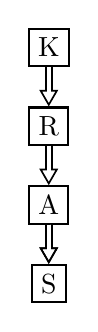
\begin{tikzpicture}[thick]
  			\node[draw,rectangle] (a) {K};
  			
	  		\node[draw,rectangle,below of=a] (b) {R};
  			\node[draw,rectangle,below of=b] (c) {A};
  			\node[draw,rectangle,below of=c] (d) {S};
			
  			% 1st pass: draw arrows
  			\draw[vecArrow] (a) to (b);
  			\draw[vecArrow] (b) to (c);
			\draw[vecArrow] (c) to (d);

  			% 2nd pass: copy all from 1st pass, and replace vecArrow with innerWhite
  			\draw[innerWhite] (a) to (b);
 		 	\draw[innerWhite] (b) to (c);
			\draw[vecArrow] (c) to (d);

  		% Note: If you have no branches, the 2nd pass is not needed
		\end{tikzpicture}
		\begin{itemize}
			\item K = kinect
			\item R = raspberry pi 2
			\item A = Arduino
			\item S = Servo controller
		\end{itemize}
		\newpage
		\textbf{Model of algorithm} \\
		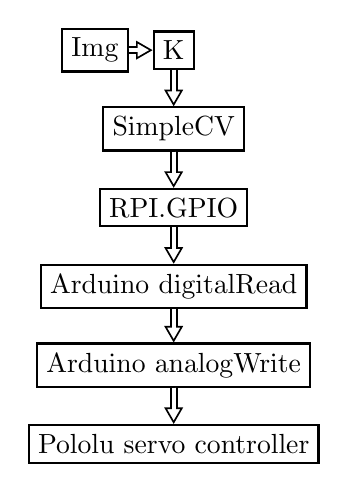
\begin{tikzpicture}[thick]
  			\node[draw,rectangle] (a) {K};
  			
	  		\node[draw,rectangle,below of=a] (b) {SimpleCV};
  			\node[draw,rectangle,below of=b] (c) {RPI.GPIO};
  			\node[draw,rectangle,below of=c] (d) {Arduino digitalRead};
			\node[draw,rectangle,left of=a] (e) {Img};
			\node[draw,rectangle,below of=d] (f) {Arduino analogWrite};
			\node[draw,rectangle,below of=f] (g) {Pololu servo controller};
			
  			% 1st pass: draw arrows
  			\draw[vecArrow] (a) to (b);
  			\draw[vecArrow] (b) to (c);
			\draw[vecArrow] (c) to (d);
			\draw[vecArrow] (e) to (a);
			\draw[vecArrow] (d) to (f);
			\draw[vecArrow] (f) to (g);

%  			% 2nd pass: copy all from 1st pass, and replace vecArrow with innerWhite
%  			\draw[innerWhite] (a) to (b);
% 		 	\draw[innerWhite] (b) to (c);
%			\draw[vecArrow] (c) to (d);
%			\draw[vecArrow] (e) to (a);
%			\draw[vecArrow] (d) to (f);
%			\draw[vecArrow] (f) to (g);

  		% Note: If you have no branches, the 2nd pass is not needed
		\end{tikzpicture}
		\begin{itemize}
			\item Img = Image
			\item K = kinect
			\item SimpleCV = Python wrappers for OpenCV
			\item RPI.GPIO = Python wrappers for controlling Raspberry Pi GPIO pins
			\item Arduino digitalRead = Arduino function to read if pin is high or low
			\item Arduino analogWrite = Arduino function for Pulse Width Modulation on capable pin
			\item Pololu servo controller = Device responsible for driving servo motors that move robot
		\end{itemize}
		\newpage
		\textbf{Raspberry Pi 2 Model B}
		\begin{itemize}
			\item Justification (Why use a raspberry pi 2 for this?)
				\begin{itemize}
					\item \textit{Mobility} \\
						We want it to be small so that it can fit inside the robot. Having to use a full size laptop with a robot limits its mobility significantly and we'd like to avoid that.
					\item \textit{More computing power than the previous version of raspberry pi} \\
						A color image consists of three two-dimensional matrices for red, green, and blue. To process this information OpenCV makes heavy use of matrix operations.
						It is important that whatever we do with OpenCV that the raspberry pi 2 can handle it.
					\item \textit{GPIO for interfacing} \\
						Our high level system design shows that the raspberry pi 2 must interface with an arduino. The arduino is then responsible for making the robot move.
						The 40-pin GPIO header on the raspberry pi 2 can be used for that very purpose. Furthermore, its even possible that the arduino can be taken out of the picture altogether.
					\item \textit{Easy to use} \\
						Raspberry pi's are very easy to set up. They come with an already optimized operating system that is capable of using all the software needed to achieve what is outlined in this report.
					\item \textit{Can be set up for remote access with USB wireless module} \\
						Raspberry pi's operating system already has a kernel driver for USB devices which means an off the shelf USB wireless module can be purchased and used for internet access.
						It is likely that additional software might need to be installed but it is also likely that the raspberry pi can handle it.
				\end{itemize}
			\item Software Dependencies
				\begin{itemize}
					\item \href{https://github.com/sightmachine/SimpleCV/tree/develop}{Simple CV}
						\begin{itemize}
							\item Elegant python wrappers for OpenCV
							\item Easy to use and can use with Kinect or regular camera (e.g. \href{https://www.raspberrypi.org/products/camera-module/}{Raspberry Pi camera module})
						\end{itemize}
					\item \href{https://github.com/OpenKinect/libfreenect}{libfreenect}
						\begin{itemize}
							\item Open source driver for Microsoft Kinect
							\item Required for using Simple CV Kinect functionality
							\item Can also be used on its own to implement Kinect functionality
						\end{itemize}
					\item \href{http://sourceforge.net/p/raspberry-gpio-python/wiki/install/}{RPi.GPIO}
						\begin{itemize}
							\item Used for controlling GPIO pins
							\item Easy to use
							\item Capable of simple operations such as Input, Output, and PWM
						\end{itemize}
				\end{itemize}
			\item Resources
				\begin{itemize}
					\item \href{http://sourceforge.net/p/raspberry-gpio-python/wiki/}{RPi.GPIO Documentation}
					\item \href{https://github.com/sightmachine/SimpleCV/blob/develop/doc/HOWTO-Install\%20on\%20RaspberryPi.rst}{Simple CV installation instructions}
					\item \href{http://openkinect.org/wiki/Getting_Started}{libfreenect installation instructions}
				\end{itemize}
		\end{itemize}
		\begin{figure}[H]
			\centering
			\caption{Raspberry Pi 2 Model B GPIO Mapping}
			\fbox{\includegraphics[scale=.3]{GPIO_Pi2.png}}
		\end{figure}
\end{description}

\end{document}